\documentclass{beamer}

%% Use package ----------------------------------------------------------------
\usepackage[T1]{fontenc}
\usepackage[utf8]{inputenc}
\usepackage{lmodern}
\usepackage{graphicx}
\usepackage[absolute,overlay]{textpos}
\usepackage{multicol}
\usepackage{listings}
\usepackage{svg}

%% Beamer customization--------------------------------------------------------

\usepackage{xcolor}
\usetheme{Warsaw}

%% Themes
% Outer themes
\useoutertheme{shadow}
% Rounded boxes and shadows
\useinnertheme[shadow=true]{rounded}
% Solid \item symbols
\useinnertheme{circles}

%% Custom colors
\definecolor{rltgreen}{rgb}{0,0.5,0}
\definecolor{pasteur}{RGB}{0,90,154}
\setbeamerfont{block title}{size={}}
\setbeamercolor{structure}{fg=pasteur}
\setbeamercolor{item}{fg=pasteur}

%Color of title
\setbeamertemplate{frametitle}
{
    \nointerlineskip
    \begin{beamercolorbox}[sep=0.3cm,ht=1.8em,wd=\paperwidth]{frametitle}
        \vbox{}\vskip-2ex%
        \strut\insertframetitle\strut
        \vskip-0.8ex%
    \end{beamercolorbox}
}
% Hide navigation symbols
\setbeamertemplate{navigation symbols}{}

%% Title block
\setbeamercolor*{title}{use=structure,fg=white,bg=pasteur}

\makeatletter

%% Top infolines
\setbeamertemplate{headline}{%
\leavevmode%
  \hbox{%
    \begin{beamercolorbox}[wd=\paperwidth,ht=2.5ex,dp=1.125ex]{palette quaternary}%
    \insertsectionnavigationhorizontal{\paperwidth}{}{\hskip0pt plus1filll}
    \end{beamercolorbox}%
  }
}

%% Define Snakemake -----------------------------------------------------------

\definecolor{eclipseBlue}{RGB}{42,0.0,255}
\definecolor{eclipseGreen}{RGB}{63,127,95}
\definecolor{eclipsePurple}{RGB}{127,0,85}

\lstset{language=Python}
\lstset{
    basicstyle=\scriptsize\ttfamily,
    morekeywords={rule, output, shell, params, run, configfile, temp, log},
    showstringspaces=false,
    commentstyle=\color{eclipseGreen}, % style of comments
    keywordstyle=\color{eclipsePurple}, % style of keywords
    stringstyle=\color{eclipseBlue}, % style of strings
}

\AtBeginSection[]{
  \begin{frame}
  \vfill
  \centering
  \begin{beamercolorbox}[sep=8pt,center,shadow=true,rounded=true]{title}
    \usebeamerfont{title}\insertsectionhead\par%
  \end{beamercolorbox}
  \vfill
  \end{frame}
}

%% Set up title ----------------------------------------------------------------

\title[Sequana]{Sequana: a set of Snakemake NGS pipelines}
\author[D.Desvillechabrol \& T.Cokelaer]{Dimitri Desvillechabrol, Rachel Legendre,
    Mélissa Cardon\\ and Thomas Cokelaer}
\date{September 25th 2017, Institut Curie, Paris}

\begin{document}

%% Title slide ----------------------------------------------------------------

\begin{frame}[plain]
    \titlepage
    \begin{textblock*}{5cm}(4.5cm,0.3cm)
        
\includegraphics[scale=0.09]{images/Institut_Pasteur.png}
    \end{textblock*}
\end{frame}



%\usebackgroundtemplate{\centering
%\includegraphics[width=\paperwidth,
%height=\paperheight]{images/strand.png}}

%\addtobeamertemplate{block 
%begin}{\pgfsetfillopacity{0.5}}{\pgfsetfillopacity{1}}
%\addtobeamertemplate{block alerted 
%begin}{\pgfsetfillopacity{0.5}}{\pgfsetfillopacity{1}}
%\addtobeamertemplate{block example 
%begin}{\pgfsetfillopacity{0.5}}{\pgfsetfillopacity{1}}


%% Slides ---------------------------------------------------------------------

\section{Introduction}

\begin{frame}
    \frametitle{Motivation}
 
 Development driven by the Biomics Pole at Pasteur Institute, which involves
 many aspects of NGS including :
 
 \tiny
 \begin{block}{https://research.pasteur.fr/en/team/biomics/}
  \begin{itemize}
  \item De novo and targeted sequencing of viruses, prokaryotes and eukaryotes
  \item Variant (SNP, indel, large rearrangements) detection
  \item Human and Mouse SNP detection by array
  \item Transcriptional analysis (RNA-Seq) for both prokaryotes and eukaryotes
  \item 16S and deep-sequencing metagenomic studies (mouse, human, and other environments)
  \item Bottom-up whole proteomic analysis and quantification
  \item Analysis of a wide range of post-translational modifications
  \item Determination of the dynamics of protein complexes.
  \item Epigenetics (CHIP-Seq, methylation studies)
  \item Projects involving two or more techniques (i.e. proteogenomics, single-cell DNA/RNA analysis)
  \end{itemize}
 \end{block}
 \small 
\end{frame}

\begin{frame}
  \frametitle{How ?}
  
  \begin{columns}
    \begin{column}{1.5cm}
      
\includegraphics[height=0.2\textheight]{images/logo_python.png} 
    \end{column}
    \begin{column}{9cm}
      A glue language, a scientific language
    \end{column}
  \end{columns}
  
  \rule{\textwidth}{1pt}
  
  \begin{columns}
    \begin{column}{1.5cm}
      
\includegraphics[height=0.2\textheight]{images/logo_snakemake.png}
    \end{column}
    \begin{column}{9cm}
      A pipeline framework mixing Python and Makefile \\
      {\footnotesize \textcolor{blue}{\textit{Köster, Johannes and Rahmann, Sven. 
      Snakemake - A scalable bioinformatics workflow engine. Bioinformatics 2012.}}}
    \end{column}
  \end{columns}
  
  \rule{\textwidth}{1pt} 
  
  \begin{columns}
    \begin{column}{1.5cm}
      
\includegraphics[height=0.2\textheight]{images/exe.png}
    \end{column}
    \begin{column}{9cm}
      Dedicated standalone such as genome coverage characterisation.\\
      {\footnotesize \textcolor{blue}{\textit{D. Desvillechabrol, C. 
      Bouchier, S. Kennedy, T. Cokelaer Detection and characterization of low 
      and high genome coverage regions .... BioRxiv 
      https://doi.org/10.1101/092478 }}}
    \end{column}
  \end{columns}
\end{frame}

\section{Snakemake}

\begin{frame}
  \frametitle{What is snakemake ?}
  
\includegraphics[scale=0.45]{images/equation.png} 
  \begin{itemize}
    \item  Clusters can be used with minimum efforts (no intrusive code)
    \item  Workflows can be run from or up to a given rule
    \item  Nice logging system to follows the status
    \item  Suspend /  Resume 
    \item  Various code can be integrated: R, bash, and of course Python
  \end{itemize}
\end{frame}

\begin{frame}[fragile]
  \frametitle{Pipeline example: minimalist (GC content)} 
  \centering
  
  \begin{columns}
    \begin{column}{7.2cm}
      \hspace{-2cm}
      \begin{lstlisting}
# list of FastQ files without extension
files = ["A", "B", ....]

rule all:
    input: expand("{data}.png", data=files), 
        "index.html"

rule create_GC_images:
    input: "{data}.fastq.gz"
    output: "{data}.png"
    run: # CODE TO COMPUTE IMAGES
        
rule html_report:
    input: expand("{data}.png", data=files)
    output: "index.html"
    run: # CODE TO CREATE HTML 
      \end{lstlisting} 
    \end{column}
    \begin{column}{3.9cm}
      \hspace{1cm}
      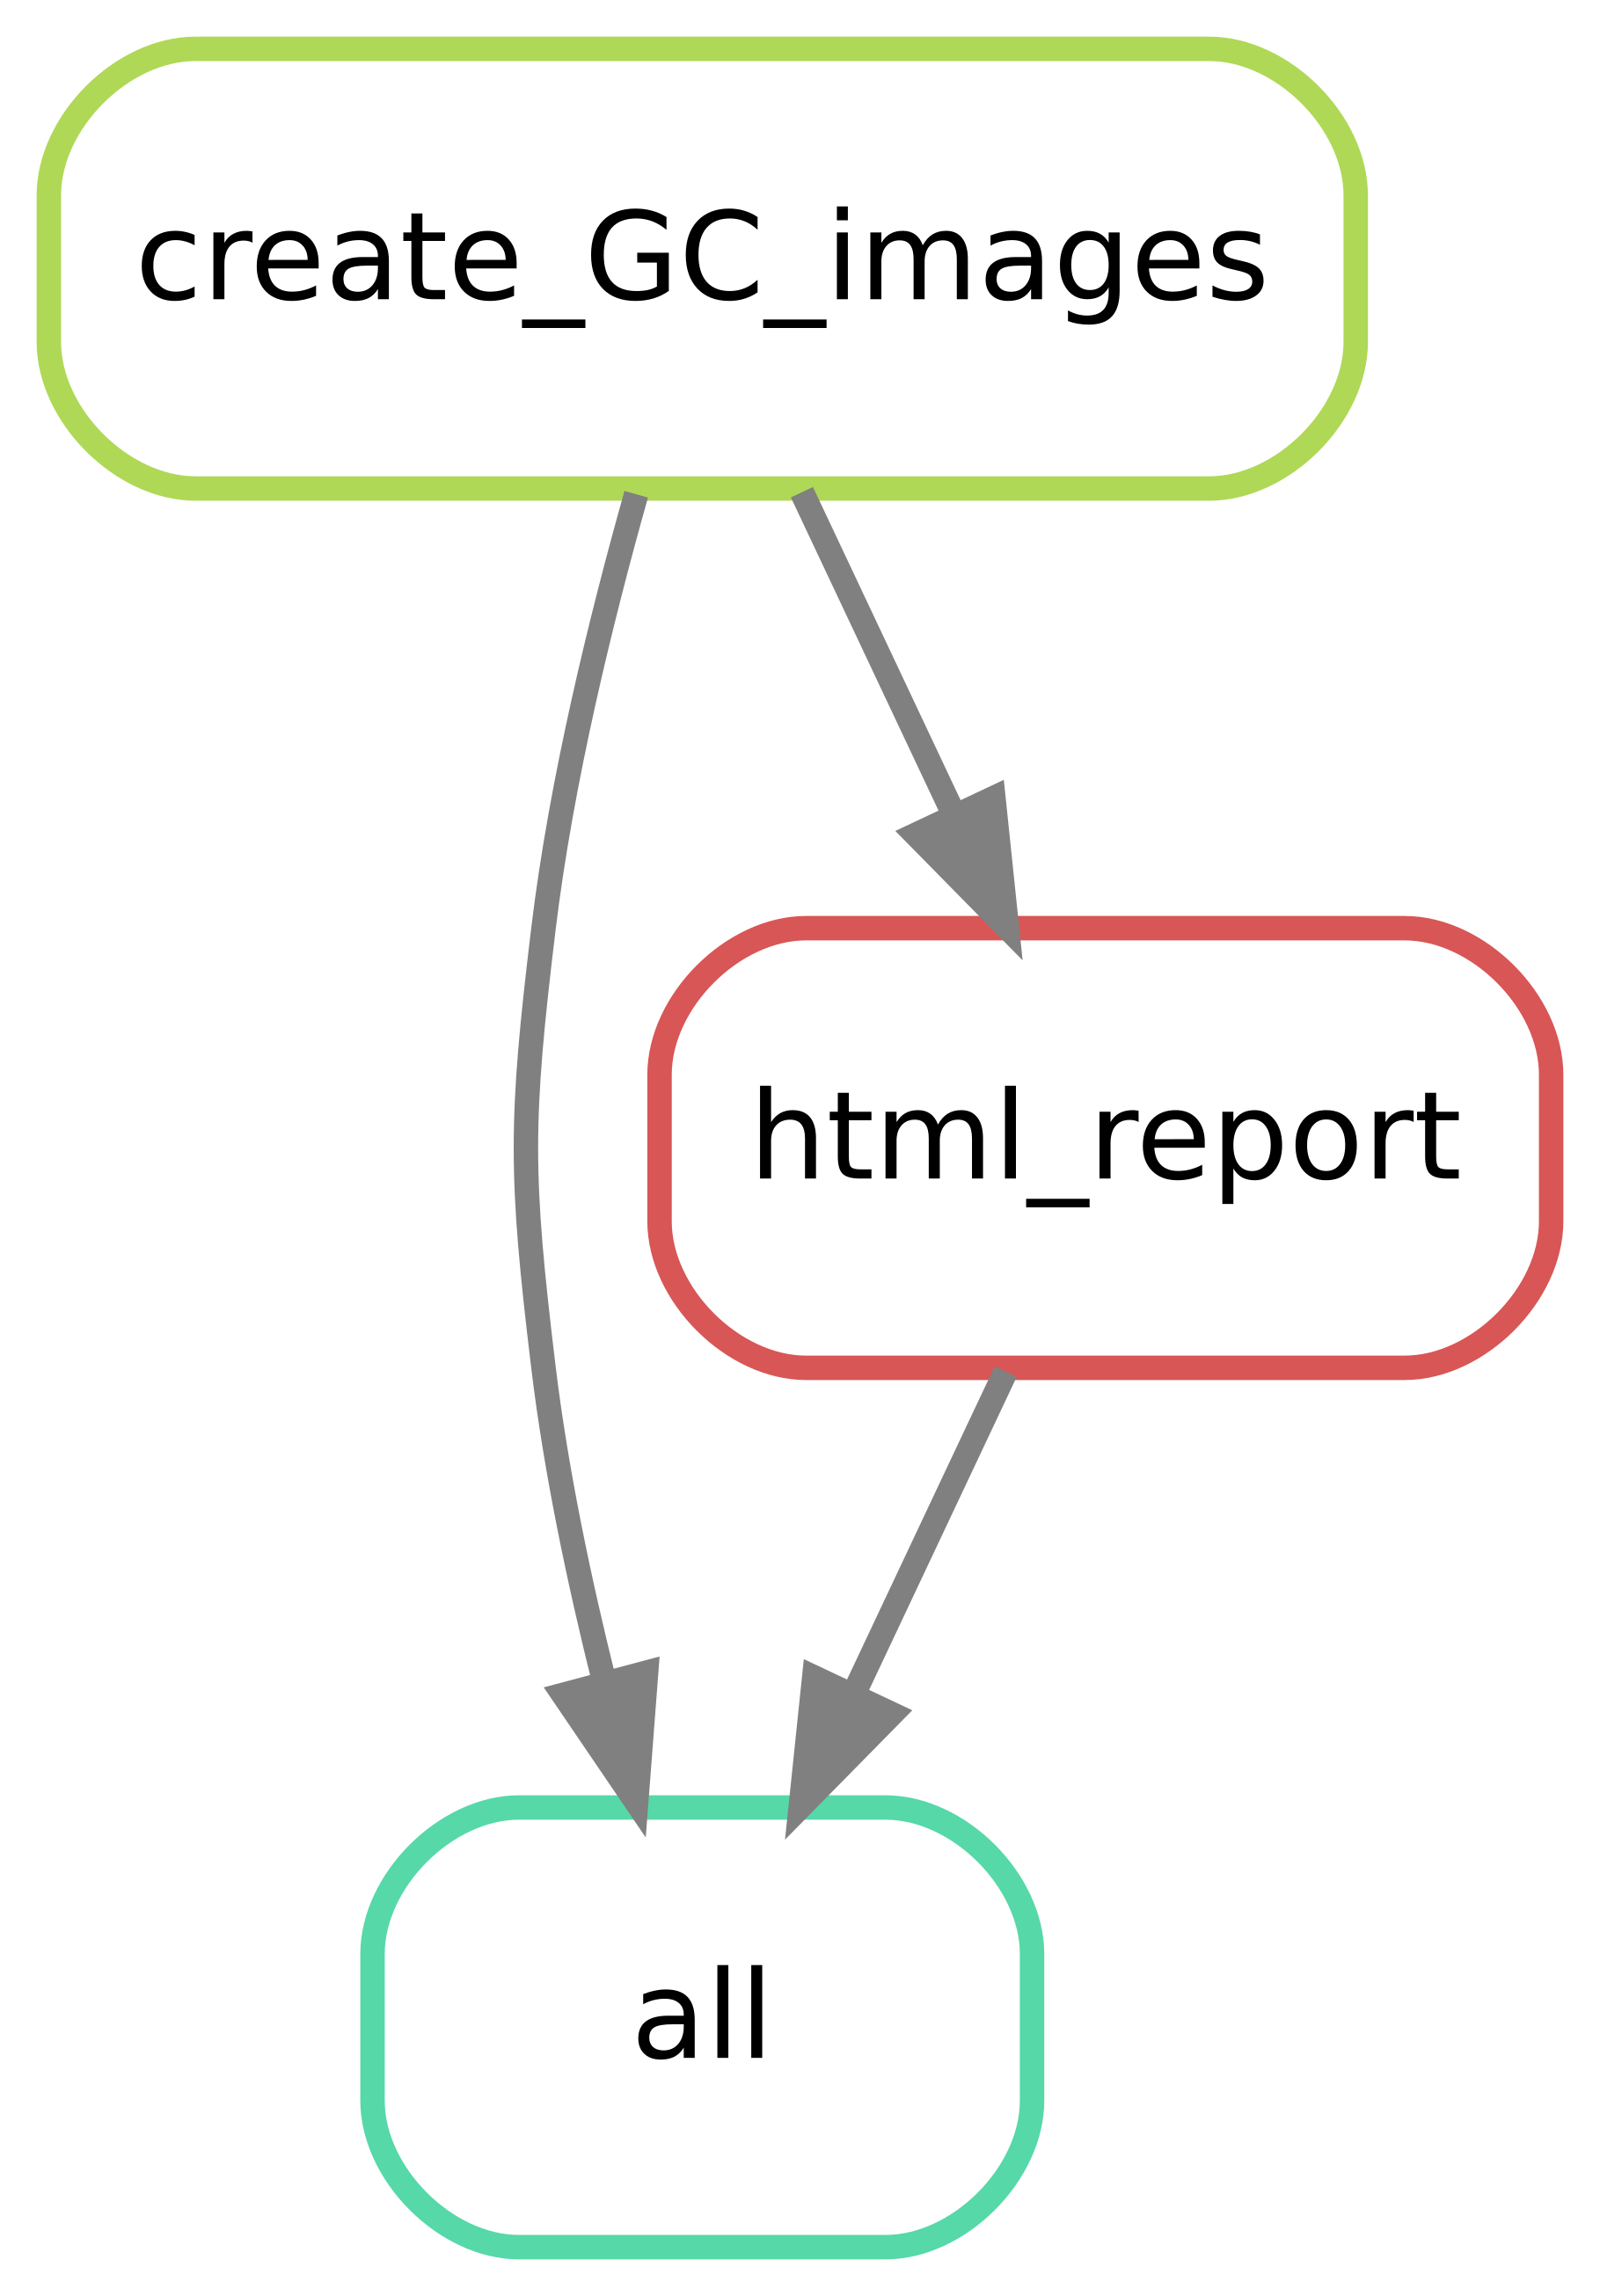
\includegraphics[scale=2.2]{./images/gc.png}
    \end{column}
  \end{columns}
\end{frame}

\begin{frame}[fragile]
  \frametitle{Execution}
  From a shell:
  \rule{\textwidth}{1pt}
  \begin{lstlisting}[basicstyle=\ttfamily\large]
snakemake -s gc_minimalist.rules
  \end{lstlisting}
  \rule{\textwidth}{1pt}
  More options if a configuration file is required, or execution is on a cluster, 
  or \dots something goes wrong.
\end{frame}


\section{Sequana}

\begin{frame}
  \frametitle{Pipelines available in Sequana}
  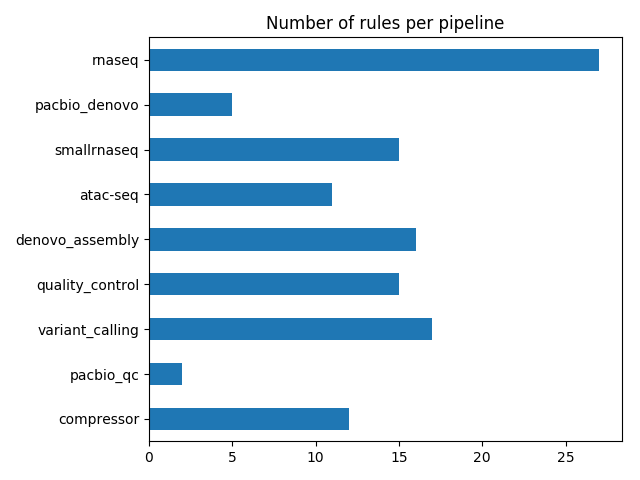
\includegraphics[scale=.6]{images/number_pipeline.png}
\end{frame}

\begin{frame}
\frametitle{Pipeline RNA-seq}
  \centering
  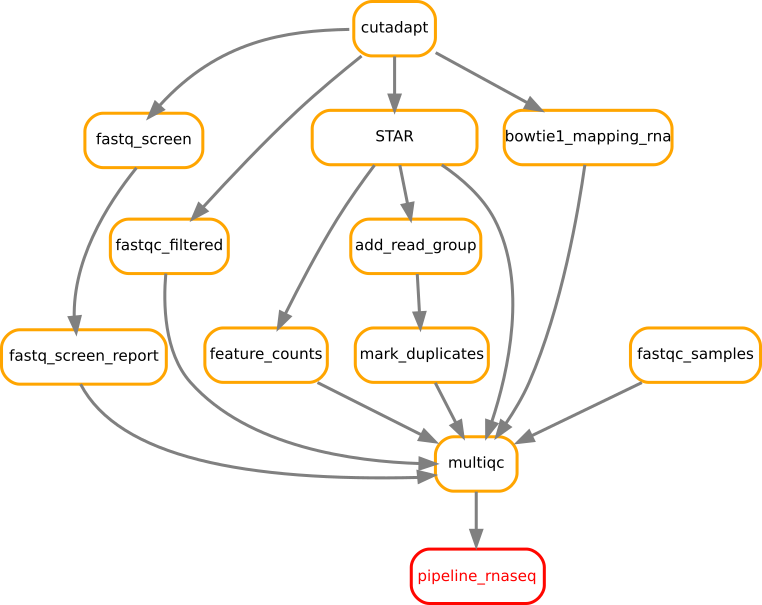
\includegraphics[scale=0.45]{./images/rnaseq.png}
\end{frame}

\begin{frame}[fragile]
  \frametitle{Markduplicates rule}
    \begin{textblock*}{15cm}(.3cm,1.5cm)
    \begin{lstlisting}
rule mark_duplicates:
    """DOCSTRING"""
    input:
        __mark_duplicates__input
    output:
        bam = __mark_duplicates__output,
        metrics = __mark_duplicates__metrics
    log:
        out = __mark_duplicates__log_std,
        err = __mark_duplicates__log_err
    params:
        remove = config["mark_duplicates"]["remove"],
        tmpdir = config["mark_duplicates"]["tmpdir"]
    shell:
        """
        (picard MarkDuplicates I={input} O={output.bam} \
            M={output.metrics} REMOVE_DUPLICATES={params.remove} \
            TMP_DIR={params.tmpdir} && samtools index {output.bam}) \
            > {log.out} 2> {log.err}
        """
  \end{lstlisting}
  \end{textblock*}
\end{frame}

\begin{frame}[fragile]
  \frametitle{Snakefile}
  \begin{textblock*}{15cm}(.3cm, 2cm)
  \begin{lstlisting}
# Mark duplicates
if config["mark_duplicates"]["do"]:
    __mark_duplicates__input = __add_read_group__output
    __mark_duplicates__output = manager.getname(
        "mark_duplicates", ".bam")
    __mark_duplicates__metrics = manager.getname(
        "mark_duplicates", ".metrics")
    __mark_duplicates__log_std = manager.getlogdir(
        'mark_duplicates_stdout.logs')
    __mark_duplicates__log_err = manager.getlogdir(
        'mark_duplicates_stderr.logs')
    include: sm.modules["mark_duplicates"]
    expected_output.extend(expand(__mark_duplicates__output,
        sample=manager.samples))
  \end{lstlisting}
  \end{textblock*}
\end{frame}

\begin{frame}[fragile]
  \frametitle{YAML configuration file}
  \begin{textblock*}{15cm}(.3cm,1.5cm)
  \begin{lstlisting}
####################################################################
# mark_duplicates (picard-tools) allows to mark PCR duplicate in 
# BAM files
#
# :Parameters:
#
# - do: if unchecked, this rule is ignored. Mandatory for RNA-SeQC
#       tool.
# - remove: If true do not write duplicates to the output file
#           instead of writing them with appropriate flags set.
#           Default value: false. This option can be set to
#           'null' to clear the default value.
#           Possible values: {true, false}
# - tmpdir: write tempory file on this directory
#           (default /tmp/)
#
mark_duplicates:
    do: yes
    remove: no
    tmpdir: "/local/scratch/"
  \end{lstlisting}
  \end{textblock*}
\end{frame}

\begin{frame}[fragile]{Using command line}
    \begin{itemize}
        \item One command line to initiate the pipeline
    \end{itemize}
    \begin{exampleblock}{Shell}
    \begin{lstlisting}[language={}]
    sequana --pipeline rnaseq \
            --input-directory path/to/sample/ \
            --reference sequence.fasta \
            --output-directory analysis/
    \end{lstlisting}
    \end{exampleblock}
    \begin{itemize}
        \item The sequana executable creates a directory with the project name
        \item The directory contains all the necessary files (config, snakefile)
    \end{itemize}
\end{frame}

\section{Sequanix}

\begin{frame}
\frametitle{Sequanix: a standalone application in PyQt}

\begin{block}{Sequanix}
\begin{itemize}
 \item Users do not want to see the Snakefile
 \item Developers do not want users to see the Snakefile
 \pause
 \item Users do not want to edit the configuration file manually
 \item Developers do not want users to edit the configuration file manually
 \pause
 \item We want a GUI that works on a local computer or on clusters.
 \pause
 \item Sequana developers want to expose their pipelines dynamically
 \pause
 \item Snakemake developers want to use Sequanix ;-) 
\end{itemize}
\end{block}
\end{frame}

\begin{frame}{GUI to simplify the usage of Snakemake pipeline}
    \begin{columns}
        \begin{column}{0.5\textwidth}

            \only<1>{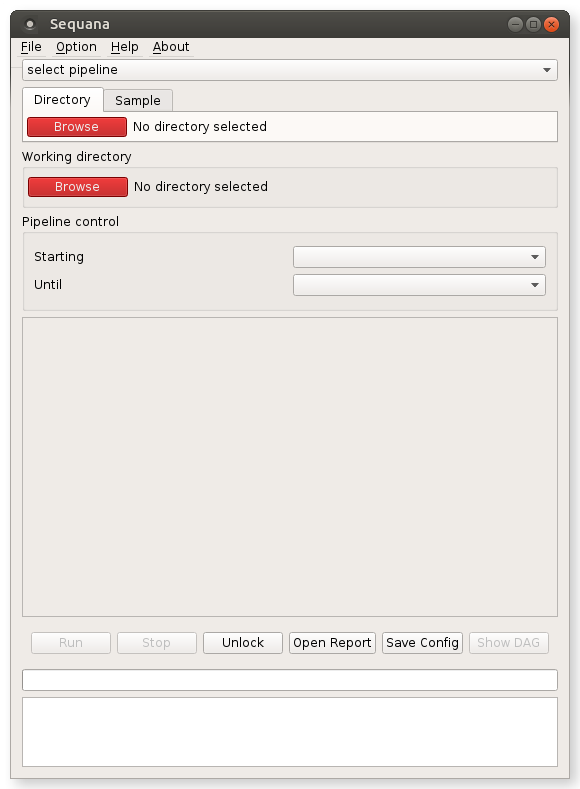
\includegraphics[scale=0.25]{../../images/sequana_init}}

            \only<2>{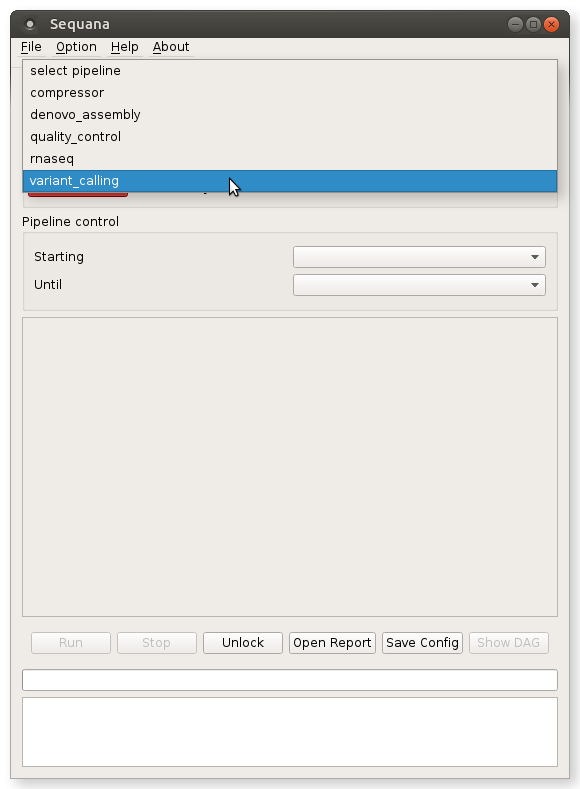
\includegraphics[scale=0.25]{../../images/choose_pipeline}}

            \only<3>{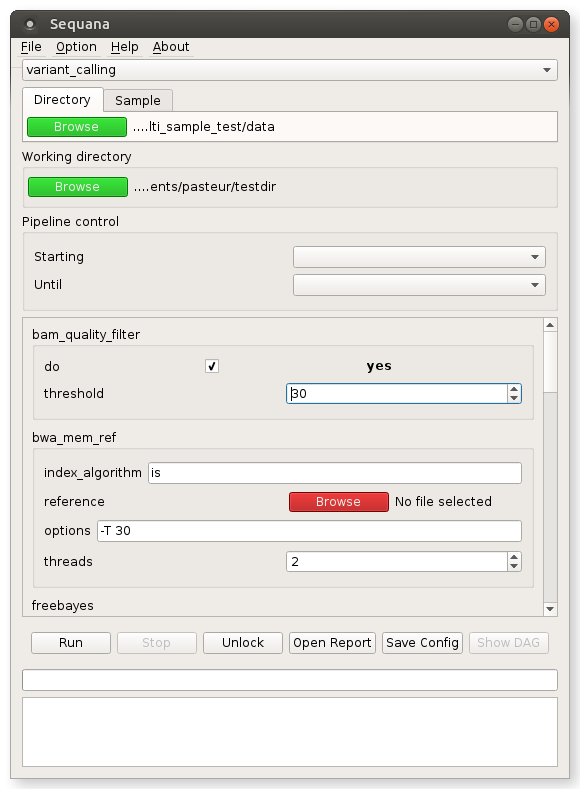
\includegraphics[scale=0.25]{../../images/choose_input_output}}

            \only<4>{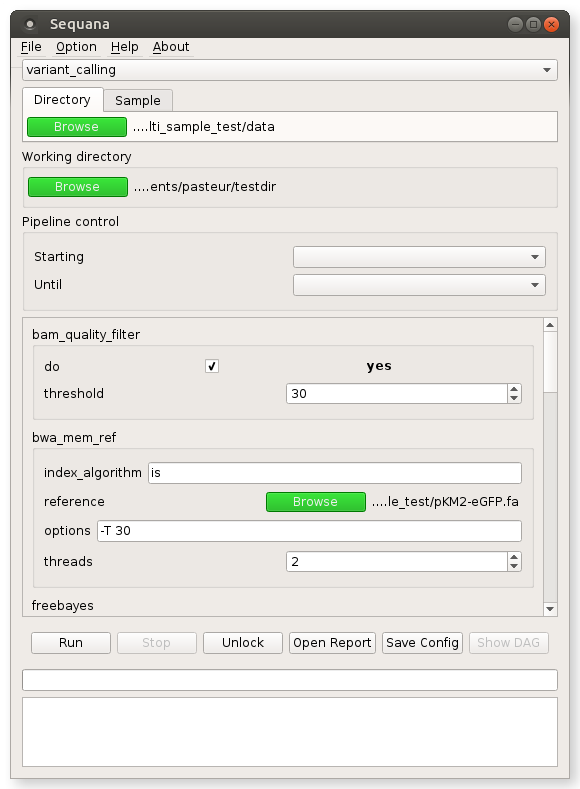
\includegraphics[scale=0.25]{../../images/sequana_pipeline}}

            \only<5>{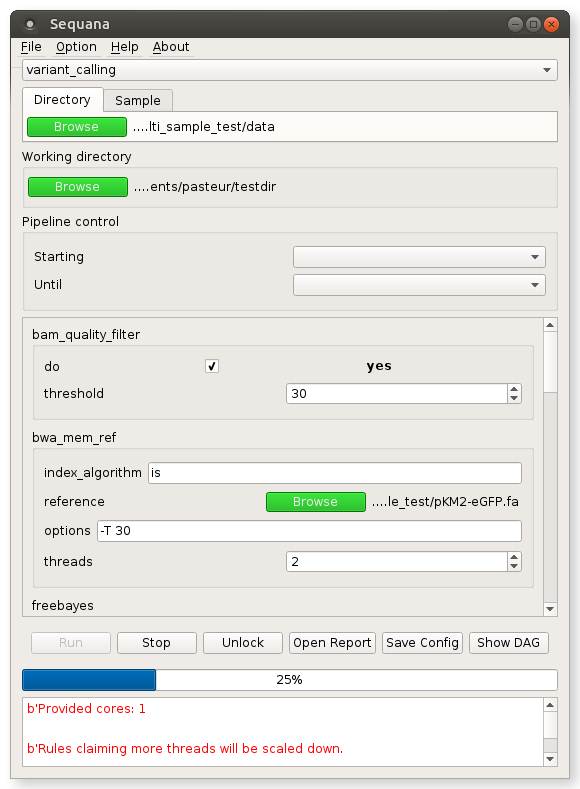
\includegraphics[scale=0.25]{../../images/sequana_running}}

            \only<6>{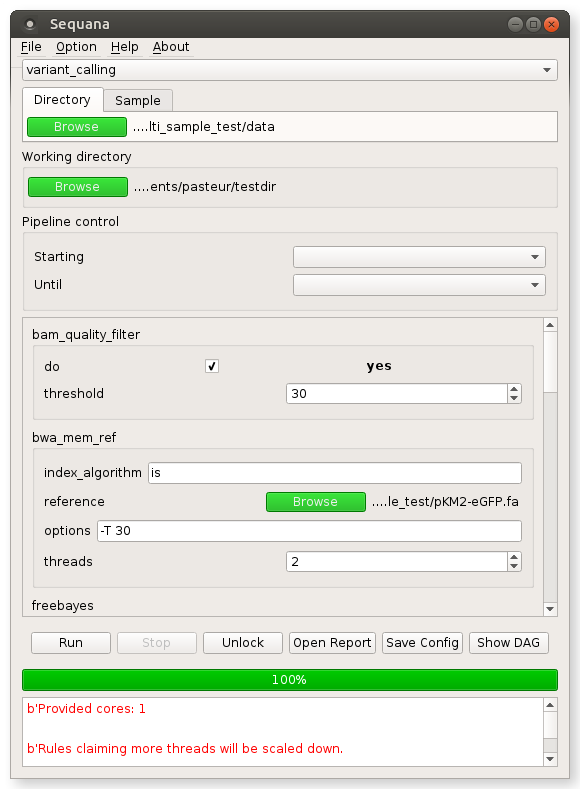
\includegraphics[scale=0.25]{../../images/sequana_finish}}

        \end{column}
        \begin{column}{0.5\textwidth}
            \only<1>{
                \begin{itemize}
                    \item Interface developed with PyQT5 and Python
                    \item Wrap our snakemake pipelines to ease the usage
                    \item Usable on our cluster, which allows X11
                \end{itemize}
            }
            \only<2-6>{
            \begin{enumerate}
                \item<2-6> Choose a pipeline
                \item<3-6> Set input and output
                \item<4-6> Fill the config form
                \item<5-6> Run the pipeline
                \item<6> Finished !
            \end{enumerate}
            }
        \end{column}
    \end{columns}
\end{frame}

\begin{frame}{Automatic tooltips}
  \centering
  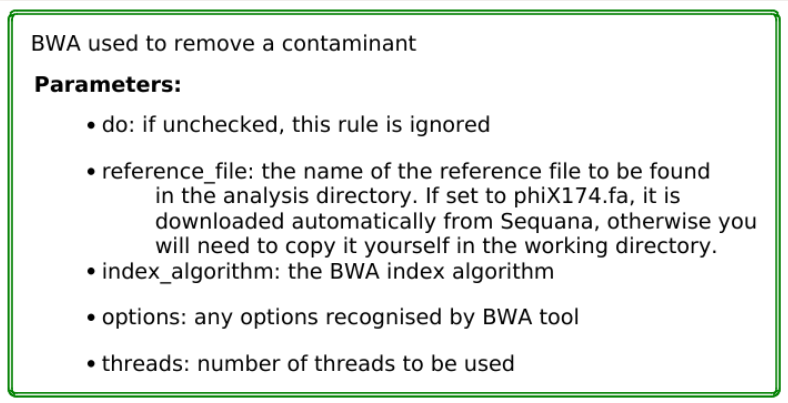
\includegraphics[scale=0.4]{images/tooltip.png}
\end{frame}

\begin{frame}{Last version of Sequanix}
  \begin{columns}
    \begin{column}{0.6\textwidth}
      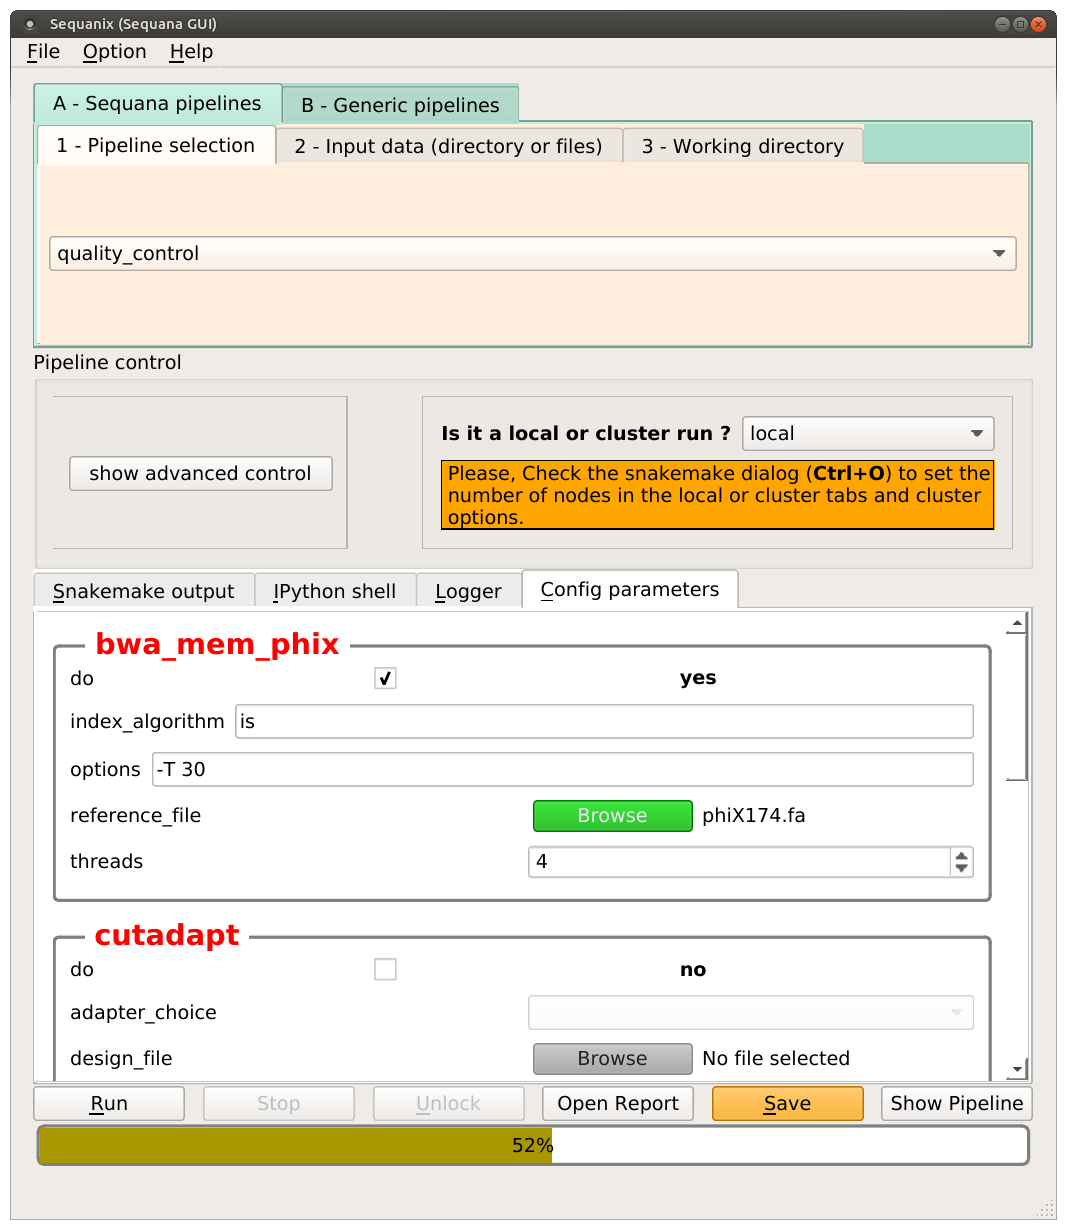
\includegraphics[scale=0.17]{images/sequanix_paused.png}
    \end{column}
    \begin{column}{0.4\textwidth}
        Desvillechabrol, D., Legendre, R., Rioualen, C., Bouchier, C., van Helden, J., Kennedy, S., \& Cokelaer, T. (2017). Sequanix: A Dynamic Graphical Interface for Snakemake Workflows. bioRxiv, 162701.
    \end{column}
  \end{columns}
\end{frame}

\section{Continuous Integration}

\begin{frame}{Versioning, Test and Documentation}
\begin{tabular}{cp{8cm}}
\vspace{0.5cm}

\includegraphics[width=0.2\textwidth,height=0.1\textheight]{../../images/logo_github.png}
& https://github.com/sequana/sequana\\

\vspace{0.5cm}

\includegraphics[width=0.2\textwidth]{../../images/logo_travis.png}&  
Continuous Integration on Travis with 100 tests with 75\% coverage\\

\vspace{0.5cm}

\includegraphics[width=0.2\textwidth]{../../images/logo_sphinx.png}& 
Uses Sphinx (RST syntax) to document the source 
code and provides user guide.\\

\vspace{0.5cm}

\includegraphics[width=0.2\textwidth]{../../images/logo_rtd.png}& 
Updated after each commits on sequana.readthedocs.io
\end{tabular}

\end{frame}

\end{document}
